%% ------------------------------------------------------------------------- %%
\chapter{Trabalhos Relacionados}
\label{cap:trabalhos-relacionados}

Muitos estudos empíricos já foram realizados para avaliar os efeitos de TDD.
Apesar de ser uma prática também focada em design, alguns trabalhos avaliam
os efeitos de TDD na qualidade externa do sistema. 
Muitos deles apresentam definições
de TDD que não levam em conta seus efeitos no design, e talvez por isso muitas das 
pesquisas em relação à prática avaliam os efeitos de TDD sobre a qualidade 
externa, algo geralmente avaliado em técnicas de testes.
Além disso, diferentemente
do que esta pesquisa propõe, muitos estudos optaram por um
maior controle no experimento, e os realizaram dentro de ambientes acadêmicos 
com estudantes dos mais diversos cursos de computação.

Janzen \cite{janzen-arch-improvement} mostrou que programadores que usam TDD na 
indústria produziram código que passaram em, aproximadamente, 50\% mais testes 
caixa-preta do que o código produzido por grupos de controle que não usavam TDD.
O grupo que usava TDD gastou menos tempo depurando. Janzen também 
apontou que a complexidade dos algoritmos era muito menor e a quantidade e
cobertura dos testes era maior nos códigos escritos com TDD.

Outros trabalhos realizados na indústria também apresentam resultados parecidos.
Um estudo feito por Maximillien e Williams \cite{max-e-williams} mostrou uma
redução de 40-50\% na quantidade de defeitos e um impacto mínimo na
produtividade quando programadores usaram TDD. Outro estudo feito por Lui e
Chan \cite{lui-e-chan} comparando dois grupos, um utilizando TDD e o outro 
escrevendo testes apenas após a implementação, mostrou uma redução significante 
no número de defeitos no grupo que utilizava TDD. 
Além disso, os defeitos que foram encontrados eram 
corrigidos mais rapidamente pelo grupo que utilizou TDD. O estudo feito por 
Damm, Lundberg e Olson \cite{damn-lundberg-e-olson} também mostra uma redução
significante nos defeitos.

O estudo feito por George e Williams \cite{george-e-williams} mostrou que,
apesar de TDD poder reduzir inicialmente a produtividade dos desenvolvedores 
mais inexperientes, o código produzido passou entre 18\% a 50\% mais em testes 
caixa-preta do que códigos produzidos por grupos que não utilizavam TDD. Esse
código também apresentou uma cobertura entre 92\% a 98\%. Uma análise
qualitativa mostrou que 87.5\% dos programadores acreditam que TDD facilitou o 
entendimento dos requisitos e 95.8\% acreditam que TDD reduziu o tempo gasto com
debug. 78\% também acreditam que TDD aumentou a produtividade da equipe. 
Entretanto, apenas 50\% dos participantes disseram que TDD ajuda a diminuir o tempo de 
desenvolvimento. Sobre qualidade, 92\% pensam que TDD ajuda a manter um
código de maior qualidade e 79\% acreditam que ele promove um design mais simples.

Turnu \textit{et al} \cite{turnu-tdd-opensouce} discutem produtividade em
projetos de código aberto. Segundo eles, a produtividade caiu quando TDD foi
adotado completamente, mas em compensação o número de problemas diminuiu 
consideravelmente.

Nagappan \cite{nagappan-ms} mostrou um estudo de caso na Microsoft e na IBM e os
resultados indicaram que o número de defeitos de quatro produtos diminuiu de 
40\% a 90\% em relação à projetos similares que não usaram TDD. Entretanto, o 
estudo mostrou também que TDD aumentou o tempo inicial de desenvolvimento entre 15\%
a 35\%. Langr \cite{langr} apontou que TDD aumenta a qualidade código, provê uma 
facilidade maior de manutenção e ajuda a produzir 33\% mais testes comparados  a
abordagens tradicionais.

Um estudo feito por Erdogmus \textit{et al} \cite{erdogmus-morisio} com 24 estudantes de
graduação mostrou que TDD aumenta a produtividade. Entretanto nenhuma diferença 
de qualidade no código foi encontrada.

Outro estudo feito por Janzen \cite{janzen-saiedian} com três diferentes grupos
de alunos (cada um deles usando uma abordagem diferente: TDD, testes depois, sem
testes), mostrou que o código produzido pelo time que fez TDD usou melhor os
conceitos de orientação a objetos e as responsabilidades foram separadas em 13 
diferentes classes, enquanto os outros times produziram um código mais
procedural. O time de TDD também produziu mais código e entregou mais
funcionalidades. Os testes produzidos por esse time teve duas vezes mais
asserções que os outros e cobriu 86\% mais branches do que o time \textit{test-last}. 
Além do mais, as classes testadas tinham valores de acoplamento 104\% menor do 
que as classes não testadas e os métodos eram, na média, 43\% menos complexos 
do que os não-testados.

Dogsa e Batic \cite{dogsa-batic} também encontraram uma melhora no
design de classes feita com TDD. Mas, segundo os autores, esse design é 
consequência da simplicidade que a prática de TDD agrega ao processo. Eles
também  afirmaram que a bateria de testes de regressão gerada durante a prática 
permite ao desenvolvedor a constante refatoração do código.

Angela Li \cite{angela-li} propôs um estudo qualitativo para
entender a eficácia de TDD. Por meio de um estudo de caso, Angela coletou as 
percepções de benefícios que praticantes de TDD têm sobre a prática. Para isso ela
fez uso de cinco entrevistas semi-estruturadas realizadas em empresas de software de 
Auckland, Nova Zelândia. Os resultados das entrevistas foram analisados e alinhados
com os maiores temas discutidos sobre o assunto na literatura: qualidade de código,
qualidade da aplicação e produtividade do desenvolvedor.
No que diz respeito à qualidade de código, Li chegou a conclusão de
que TDD guia o desenvolvedor para classes mais simples e com melhor design. 
Além disso, o código tende a ser mais simples e fácil de ler.
De acordo com o trabalho, os principais fatores que contribuem para esses benefícios
é a maior confiança em refatorar e modificar código, uma maior cobertura de testes,
entendimento mais profundo dos requisitos, maior facilidade na compreensão do código,
grau e escopo de erros reduzidos, além de uma maior satisfação pessoal do desenvolvedor.

O praticante de TDD geralmente faz uso de outras práticas ágeis, como
programação pareada, que podem dificultar o processo de avaliação dos benefícios
de TDD. Madeyski \cite{madeyski-package-dependencies} observou os resultados
entre grupos que praticavam TDD, programação pareada, e a combinação entre elas,
e não conseguiu mostrar grande diferença entre equipes que utilizam programação 
pareada e equipes que utilizam TDD, no que diz respeito à dependência entre 
pacotes. Entretanto, ao combinar os resultados, Madeyski encontrou que TDD pode 
ajudar no nível de gerenciamento de dependências entre classes. Segundo ele, o 
programador deve utilizar TDD, mas ficar atento a possíveis problemas de design.

O estudo de Muller e Hagner \cite{muller-e-hagner} apontou que TDD não resulta
em melhor qualidade ou produtividade. Entretanto, os estudantes perceberam um 
melhor reúso dos códigos produzidos com TDD. Steinberg \cite{steinberg} mostrou
que código produzido com TDD é mais coeso e menos acoplado. Os estudantes também
reportaram que os defeitos eram mais fáceis de serem corrigidos. A pesquisa feita
por Edwards \cite{edwards}, com 59 estudantes, mostrou que o código produzido com
TDD tem 45\% menos defeitos e faz o programador se sentir mais a vontade
com ele.

Aprender TDD também não é tarefa fácil. Mugridge \cite{mugridge} identificou
dois desafios principais em ensinar TDD nos últimos dois anos: fazer os estudantes
pensarem novamente sobre o design, e fazê-los se envolver com essa nova
abordagem. Além disso, é difícil fazê-los entender testes de unidade, design e refatoração
de maneira explícita. Contudo, segundo Proulx \cite{proulx}, a partir do momento que
o estudante aprende TDD, ele tende a ter uma melhor performance em disciplinas
de orientação a objetos. Segundo ele, essa melhora é percebida inclusive pelos
empregadores desses alunos. 

Outras compilações de estudos sobre TDD também podem ser encontrados no livro
\textit{Test-Driven Development: An Empirical Evaluation of Agile Practice},
escrito por Madeyski \cite{madeyski-livro} ou no trabalho entitulado
\textit{Test driven development: empirical body of evidence}, feito por
Siniaalto \cite{tdd-body-of-evidence}.

%% ------------------------------------------------------------------------- %%
\section{Discussão}

Como visto anteriormente, poucos trabalhos avaliam os efeitos de TDD sobre o
design de classes. Quando o fazem, apenas discutem quais os resultados da prática
dentro do ciclo, e não exatamente \textbf{como} TDD os influencia. Josefsson
\cite{josefsson}, em sua discussão sobre a necessidade de uma fase de desenho
arquitetural e os efeitos de TDD nesse quesito, chega à mesma conclusão. Segundo
ele, os estudos sobre TDD encontrados na literatura atual são muito limitados e
não podem ser generalizados. Por esse motivo, os ditos efeitos que TDD têm 
sobre o design não podem ser provados. Apesar desse artigo ser datado de 2004, e
muitos trabalhos terem sido realizados após essa data, o pesquisador ainda acredita 
que os efeitos de TDD ainda não foram provados pela literatura atual.

Grande parte desses estudos também não levam em conta a experiência do
programador que está praticando TDD. Geralmente esse ponto é discutido apenas 
na seção de ameaças a validade do estudo. Janzen, em seu doutorado, percebeu que
desenvolvedores mais maduros obtêm mais benefícios de TDD, escrevendo classes
mais simples. Além disso, desenvolvedores maduros que experimentam a prática
tendem a escolher TDD mais facilmente do que desenvolvedores menos experientes
\cite{janzen-phd}.

Os trabalhos que analisam TDD do ponto de vista de design, no entanto, não
chegam a resultados conclusivos; muitos deles inclusive dizem que os efeitos
de TDD não são tão diferentes daqueles dos times que não praticam TDD.  A própria tese de
doutorado de Janzen foi inconclusiva no que diz respeito à influência de TDD no 
acoplamento e na coesão \cite{janzen-phd}. 

Ao calcular LCOM-HS, métrica que tenta medir a falta de coesão de determinada
classe, não se deve levar em consideração \textit{getters} e \textit{setters} de
classes Java, por exemplo, pois esses métodos tipicamente confundem a métrica.
Acoplamento, por sua vez, é geralmente medido e comparado com os valores
obtidos em times que não praticam TDD. Os problemas desse tipo de medição é que,
em softwares complexos, é impossível não existir acoplamento, e, assim, a busca por
baixo acoplamento deve existir. Porém, tão ou mais importante do que isso, é
analisar o tipo do acoplamento: acoplar-se com classes estáveis é menos
problemático do que acoplar com classes que mudam frequentemente
\cite{bob-martin}. 

Além disso, outro ponto fortemente relacionado com design é a simplicidade e
facilidade de evolução. Um design rígido, que não permite mudanças de maneira
fácil, é difícil de ser medido de maneira quantitativa. Complexidade
desnecessária também é totalmente subjetiva. 

Portanto, a crítica dessa pesquisa
com relação aos trabalhos relacionados é justamente na análise feita sobre os
efeitos da prática no TDD. É necessário mais do que uma comparação analítica; o
ponto de vista dos desenvolvedores, que atuam naquele código-fonte durante todo
o dia de trabalho deve ser levado em consideração.

%% ------------------------------------------------------------------------- %%
\section{Posição desta pesquisa na literatura atual}

Esta pesquisa se mostra diferente da maioria dos trabalhos encontrados na
literatura atual. Além de observar TDD pelo ponto de vista única e
exclusivamente do design, colhe-se informações baseadas no ponto de
vista de desenvolvedores que a praticam.

Talvez o trabalho mais parecido com o que é proposto aqui é o
realizado por Angela Li, em 2009, que apresenta um estudo qualitativo sobre os
efeitos de TDD no processo de desenvolvimento de software \cite{angela-li}. 
A diferença é que esta pesquisa se concentra em entender e aprofundar nos
efeitos de TDD apenas no design de classes.

O caminho em destaque da Figura \ref{fig:posicao-pesquisa} mostra a nossa posição
em relação ao que já é encontrado na literatura.

\begin{figure}[h!]
  \centering
  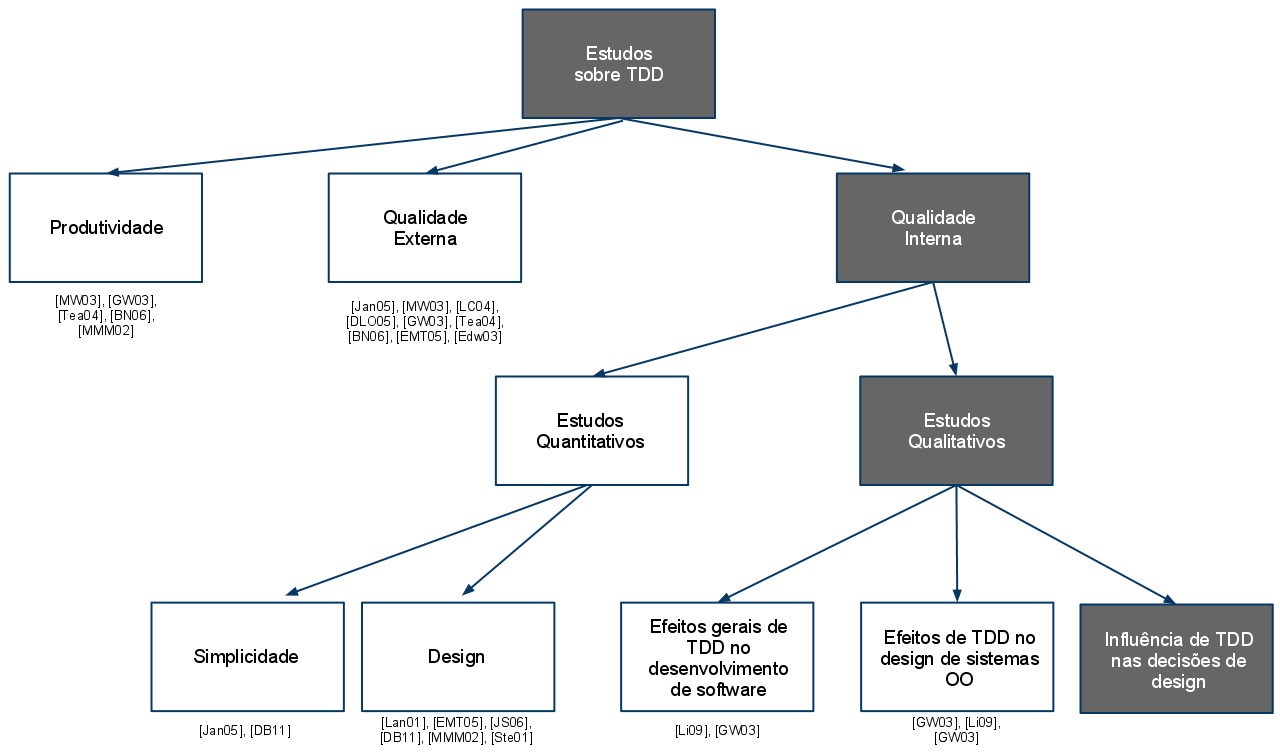
\includegraphics[scale=0.35]{posicao-pesquisa.png}
  \caption{Posição desta pesquisa na literatura atual}
  \label{fig:posicao-pesquisa}
\end{figure}

